\chapter{Machine Language Monitor}

\section{Introduction}

Before we go any further, it is important to remember that the MEGA65 typically
has two separate machine language monitors:  The one included in C65 ROMs, and
the one that is part of the Matrix Mode debug interface.  It is also possible to
replace the standard C65 monitor in the ROM with the enhanced MEGA65 OpenROMs
machine language monitor, which corrects many bugs and adds many new features --
including support for all enhanced CPU instructions of the MEGA65.  This chapter
describes all three of these machine language monitors.

\section{C65 ROM Standard Machine Language Monitor}
\index{MONITOR!Standard C65 ROM Monitor}
The machine language monitor is a debugging tool for machine language
programs. It includes a mini-assembler, a disassembler and many useful commands.
When the program execution encounters the code 00 (zero) alias BRK,
the default action of the operating system is, to call the monitor.
This features allows the debugging of programs by setting breakpoints.

\subsection{Table of C65 ROM Standard Monitor Commands}

{
\ttfamily
\setlength{\tabcolsep}{1mm}
\begin{center}
\begin{tabular}{|l|l|l|}
\hline
C & mnemonic & description \\
\hline
A &     ASSEMBLE        & Assemble a line of 45GS02 code\\
C &     COMPARE         & Compare two sections of memory\\
D &     DISASSEMBLE     & Disassemble a line of 45GS02 code\\
F &     FILL            & Fill a section of memory with a value \\
G &     GO              & Start execution at specified address\\
H &     HUNT            & Find specified data in a section of memory\\
L &     LOAD            & Load a file from disk\\
M &     MEMORY          & Dump a section of memory\\
R &     REGISTERS       & Display the contents of the 45GS02 registers\\
S &     SAVE            & Save a section of memory to a disk file\\
T &     TRANSFER        & Transfer memory to another location\\
V &     VERIFY          & Compare a section of memory with a disk file\\
X &     EXIT            & Exit Monitor mode\\
\hline
 . &     <period>        & Assembles a line of 45GS02 code\\
 > &     <greater>       & Modifies memory\\
 ; &     <semicolon>     & Modifies register contents\\
 @ &     <at sign>       & Disk command, directory or status\\
\hline
\$ &     <hex>           & Display hex, decimal, octal, and binary value \\
 + &     <decimal>       & Display hex, decimal, octal, and binary value\\
\& &     <octal>         & Display hex, decimal, octal, and binary value\\
\% &     <binary>        & Display hex, decimal, octal, and binary value\\
\hline
\end{tabular}
\end{center}
}

\subsection {Calling the Monitor}

To enter the monitor from BASIC, type:
\screentext{MONITOR}

The monitor responds with a display of register contents and waits for a command:

\begin{tcolorbox}[colback=blue,coltext=white]
\verbatimfont{\codefont}
\begin{verbatim}
MONITOR
    PC   SR AC XR YR ZR BP SP
; 000000 00 00 00 00 00 00 F8
\end{verbatim}
\end{tcolorbox}

\subsection{addresses and numbers}

All addresses and numbers must be numbers of base 16 (hex),
10 (decimal), 8 (octal) or 2 (dual). Symbolic names like CHROUT
or arithmetics like \$1000+5 are not allowed.

It is an old tradition since the first monitor of the Commodore PET,
that the default base is 16. In fact the old monitors would not
accept any other numbers, than hexadecimal (short hex).
This may confuse beginners, because a statement like
\begin{verbatim}
LDA #10
\end{verbatim}
loads the decimal value 16 into the accumulator.
Later monitors, like that of the Commodore 128 accepted numbers of
base 16,10,8 and 2 - like this one, but still used 16 (hex) as default.
Additionally the MEGA65 monitor allows character entry, which uses
the PETSCII value of the character.
Following prefixes can be used to specify the base of the following number:

{\ttfamily
{\setlength{\tabcolsep}{1mm}
\begin{center}
\begin{tabular}{|l|l|l|l|l|}
\hline
 base  & name & prefix & digits characters & example     \\
\hline
16 & hexadecimal  &     & 0123456789ABCDEF &   100       \\
16 & hexadecimal  & \$  & 0123456789ABCDEF & \$100       \\
10 & decimal      &  +  & 0123456789       & +256        \\
 8 & octal        & \&  & 01234567         & \&400       \\
 2 & dual         & \%  & 01               & \%100000000 \\
   & character    &  '  & all              & 'A          \\
\hline
\end{tabular}
\end{center}
}
}


% ======================================
% Start of the monitor command reference
% ======================================

\titleformat*{\subsubsection}{\normalfont\huge\bfseries\color{blue}}

% ***********
% DISASSEMBLE
% ***********

\subsubsection{D : DISASSEMBLE}
\index{DISASSEMBLE}
\index{MONITOR Commands!DISASSEMBLE}
\begin{description}[leftmargin=2cm,style=nextline]
\item [Format:] {\bf D [from [,to]]}
\item [Usage:] Prints a machine language listing for the specified
               address range assuming, that it contains code.
               If only one argument is present, the disassembler
               disassembles the next 21 bytes. If no argument is
               given, the disassembly continues with the last used
               disassemble address.
               The contents are printed as hex values.

\item [Remarks:] The rows start with the dot character '.'.
                 This enables direct full screen editing of the disassembly.
                 Typing return in any row will assemble the changed
                 command of the cursor row back to memory, if writable RAM is there.
                 See monitor command {\bf .}.

                 The disassembler knows the instruction set of the C65 CPU
                 GS6502. Enhanced instructions from the 45GS02 CPU of the MEGA65
                 are not recognised.

\item [Example:] Using {\bf D}
\end{description}

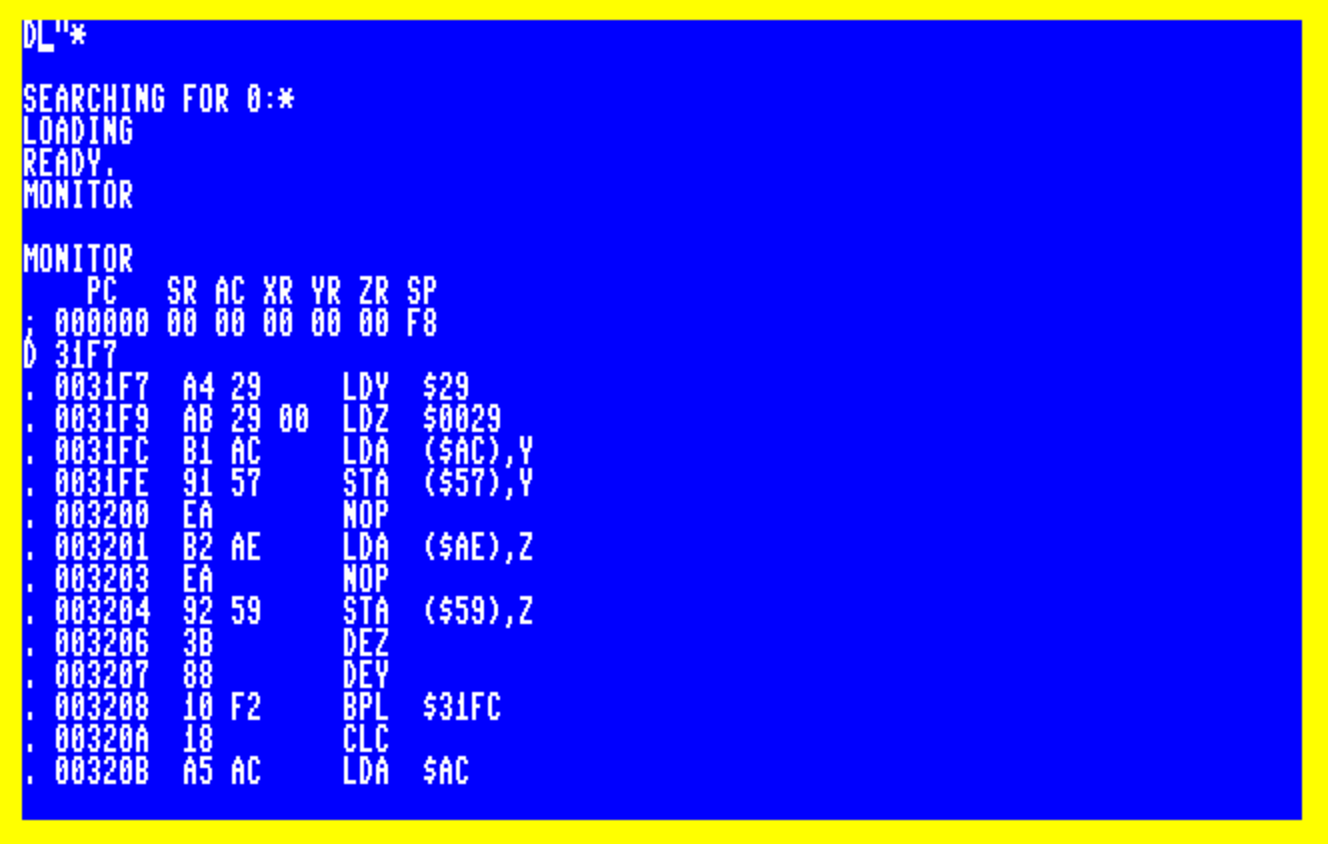
\includegraphics[width=\linewidth]{images/monitor-d}

% ******
% MEMORY
% ******

\subsubsection{M : MEMORY}
\index{MEMORY}
\index{MONITOR Commands!MEMORY}
\begin{description}[leftmargin=2cm,style=nextline]
\item [Format:] {\bf M [from [,to]]}
\item [Usage:] Prints a memory dump for the given address range.
               The dump displays memory contents, organised in rows
               of 16 consecutive addresses starting with the
               address, given as 1st. argument. The dump continues
               until a row has been printed, containing the value
               of the address given as 2nd. argument.
               If no 2nd. argument is present, the dump displays
               a full page of 256 bytes in 16 rows.
               The contents are printed as 16 byte values in hex,
               followed by the character representation.

\item [Remarks:] The rows start with the character '>'.
                 This enables direct full screen editing of the dump.
                 Typing return in any row will write the changed
                 values of the cursor row back to memory, if writable RAM is there.
                 See monitor command {\bf >}.

\item [Example:] Using {\bf M}
\end{description}

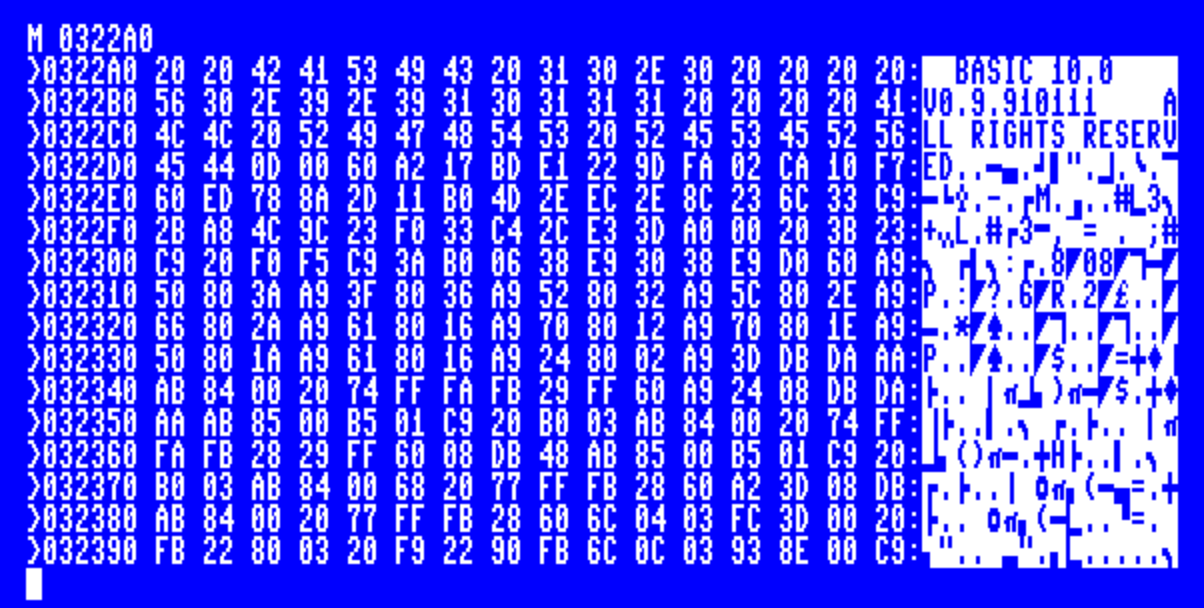
\includegraphics[width=\linewidth]{images/monitor-m}

\section{Enhanced Machine Language Monitor}
\index{MONITOR!Enhanced MEGA65 ROM Monitor}
\label{cha:MLMonitor}

This machine language monitor is a new development for the MEGA65.
It is available both in the {\tt 92XXXX} ROMs and in the OpenROMs.

The enhanced monitor has following additional features:
\begin{description}[leftmargin=1cm,style=nextline]
\item[Adddresses:] All addresses are used as 32-bit (4 bytes) addresses.
   This allows access to the whole MEGA65 address range, which needs
   28-bit. This is especially useful for the access to the 8MB RAM blocks
   called attic RAM at \$8000000 (builtin) and cellar RAM at
   \$8800000 (optional). Setting bit 31 of an address to 1 gives access
   to a special (banked) configuration. In this case the I/O area at \$D000
   and the ROM area \$6000 - \$7FFF (monitor ROM) and \$E000 - \$FFFF
   (kernal ROM) overlay the current bank.

\item[Commands:] The additional command {\bf B} displays character bitmaps.

\item[Disk access:] The disk command character {\bf \@} knows two more
  functions: {\bf U1} for reading a sequence of disk blocks to memory and
  {\bf U2} for writing a memory range to disk blocks. This enables disk
  disk editing, for example modifying directory entries or can be even
  used to backup whole floppy contents or disk images. The attic RAM is
  large enough to hold the contents of 8 complete 1581 floppies.

\item[Disassembler:] The disassembler can decode all additional
  address modes, like the 32-bit indirect mode $[\$nn],Z$
  and the compound instructions involving the use of the 32-bit Q register.

\item[Register:] The register displays the full 16-bit stack pointer
 and the base page register and accepts new settings for ithem.

\end{description}

\subsection{Table of MEGA65 Enhanced Monitor Commands}

{
\ttfamily
\setlength{\tabcolsep}{1mm}
\begin{center}
\begin{tabular}{|l|l|l|}
\hline
C & mnemonic & description \\
\hline
A &     ASSEMBLE        & Assemble a line of 45GS02 code\\
B &     BITMAPS         & Display 8x8 bitmaps (characters)\\
C &     COMPARE         & Compare two sections of memory\\
D &     DISASSEMBLE     & Disassemble a line of 45GS02 code\\
F &     FILL            & Fill a section of memory with a value \\
G &     GO              & Start execution at specified address\\
H &     HUNT            & Find specified data in a section of memory\\
L &     LOAD            & Load a file from disk\\
M &     MEMORY          & Dump a section of memory\\
R &     REGISTERS       & Display the contents of the 45GS02 registers\\
S &     SAVE            & Save a section of memory to a disk file\\
T &     TRANSFER        & Transfer memory to another location\\
V &     VERIFY          & Compare a section of memory with a disk file\\
X &     EXIT            & Exit Monitor mode\\
\hline
 . &     <period>        & Assembles a line of 45GS02 code\\
 > &     <greater>       & Modifies memory\\
 ; &     <semicolon>     & Modifies register contents\\
 @ &     <at sign>       & Disk command, directory or status\\
\hline
\$ &     <hex>           & Display hex, decimal, octal, and binary value \\
 + &     <decimal>       & Display hex, decimal, octal, and binary value\\
\& &     <octal>         & Display hex, decimal, octal, and binary value\\
\% &     <binary>        & Display hex, decimal, octal, and binary value\\
\hline
\end{tabular}
\end{center}
}


\subsection {Calling the Monitor}

To enter the monitor from BASIC, type:
\screentext{MONITOR}

The monitor responds with a display of register contents and waits for a command:

\begin{tcolorbox}[colback=blue,coltext=white]
\verbatimfont{\codefont}
\begin{verbatim}
MONITOR
\end{verbatim}
\begin{tcolorbox}[colback=yellow,coltext=blue,,arc=0mm,boxrule=0mm,
       left*=0.5mm,right*=0mm,top=0mm,bottom=0mm,nobeforeafter,
       left skip=0.1mm,
       width=50mm,height=3mm,valign=center]
\begin{verbatim}
BS MONITOR COMMANDS:ABCDFGHJMRTX@.>;?$+&%'LSV
\end{verbatim}
\end{tcolorbox}
\begin{verbatim}
    PC   SR AC XR YR ZR BP  SP  NVEBDIZC
; 00CFA4 35 00 00 00 00 00 01F8 --11-1-1
\end{verbatim}
\end{tcolorbox}

\subsection{addresses and numbers}

All addresses and numbers must be numbers of base 16 (hex),
10 (decimal), 8 (octal) or 2 (dual). Symbolic names like CHROUT
or arithmetics like \$1000+5 are not allowed.

It is an old tradition since the first monitor of the Commodore PET,
that the default base is 16. In fact the old monitors would not
accept any other numbers, than hexadecimal (short hex).
This may confuse beginners, because a statement like
\begin{verbatim}
LDA #10
\end{verbatim}
loads the decimal value 16 into the accumulator.
Later monitors, like that of the Commodore 128 accepted numbers of
base 16,10,8 and 2 - like this one, but still used 16 (hex) as default.
Additionally the MEGA65 monitor allows character entry, which uses
the PETSCII value of the character.
Following prefixes can be used to specify the base of the following number:

{\ttfamily
{\setlength{\tabcolsep}{1mm}
\begin{center}
\begin{tabular}{|l|l|l|l|l|}
\hline
 base  & name & prefix & digits characters & example     \\
\hline
16 & hexadecimal  &     & 0123456789ABCDEF &   100       \\
16 & hexadecimal  & \$  & 0123456789ABCDEF & \$100       \\
10 & decimal      &  +  & 0123456789       & +256        \\
 8 & octal        & \&  & 01234567         & \&400       \\
 2 & dual         & \%  & 01               & \%100000000 \\
   & character    &  '  & all              & 'A          \\
\hline
\end{tabular}
\end{center}
}
}

\subsection{Assembler}

The monitor has a builtin mini-assembler, which can be used to write
machine language code using the standard mnemonics like {\bf LDA} or
{\bf STA}, etc.
The most important difference to a full assembler is the necessity
to use numeric constants as operands for the instructions only.
So you cannot use named variables, labels or subroutine names.
A call to the kernal routine, which prints a character to the screen
would be written {\ttfamily {\bf JSR CHROUT}} in a full assembler, while
the mini-assembler needs the syntax {\ttfamily \bf JSR FFD2} (you need
to know or lookup the addresses). There is the convenience for
branch instructions, that the target address is written to the
operand field and the mini-assembler computes the relative address,
that is inserted in the code.

The assembler knows all instructions and address modes of the MEGA65
CPU 45GS02 (except the instructions using the Q register, these will
be added later). So an instruction like {\ttfamily \bf LDA [TXTPTR],Z}
will be assembled as loading the accumulator using a 32-bit pointer
at the addresses {\ttfamily \bf TXTPTR, TXTPTR+1, TXTPTR+2, TXTPTR+3}.

% ********
% ASSEMBLE
% ********

\subsubsection{A : ASSEMBLE}

\index{ASSEMBLE}
\index{MONITOR Commands!ASSEMBLE}
\begin{description}[leftmargin=2cm,style=nextline]
\item [Format:] {\bf A address mnemonic operand}
\item [Usage:] The mini assembler allows entry of machine language instructions
               using easy to remember mnemonics instead of opcodes.
               The operand may be entered as hex, decimal, binary or character.
               Branch targets are automatically converted to relative distances.
               After each entered instruction, the mini assembler generates
               the 1-3 byte long machine code, prints this code along with the
               instruction and advances the program counter. A new line
               is generated with the command {\bf A} and the new value of the
               program counter printed. This eases the fast entry of instructions.
               The assembly input mode is stopped by pressing RETURN only.
               Any line of the entered code or a line in disassembly format
               can be changed by moving the cursor into that line and changing
               the desired element, for example the mnemonic or the operand.
               Listed hex values before the mnemonic are ignored.

               If the monitor shall be reentered after executing the code,
               the last instruction must be a {\bf BRK} instruction
               and the program must be called with I/O and monitor ROM active.
               This is done by setting the bit 31 of the execution address.
               If the program was entered in bank 0 on address 1500,
               it should be started with: \screentext{G 80001500}.

               If the entered code is a subroutine, it must end with a
               {\bf RTS} instruction.

\item [Remarks:] The assembler recognises all 45GS02 instructions of the
                 MEGA65, except the instructions, that use the Q register.
                 These instructions can be entered by typing
                 the NEG NEG prefix explicit. E.g. instead of LDQ \$1234,
                 entering the 3 instructions (on 3 different rows)
                 NEG NEG LDA \$1234 is assembled to the equivalent code.

\end{description}
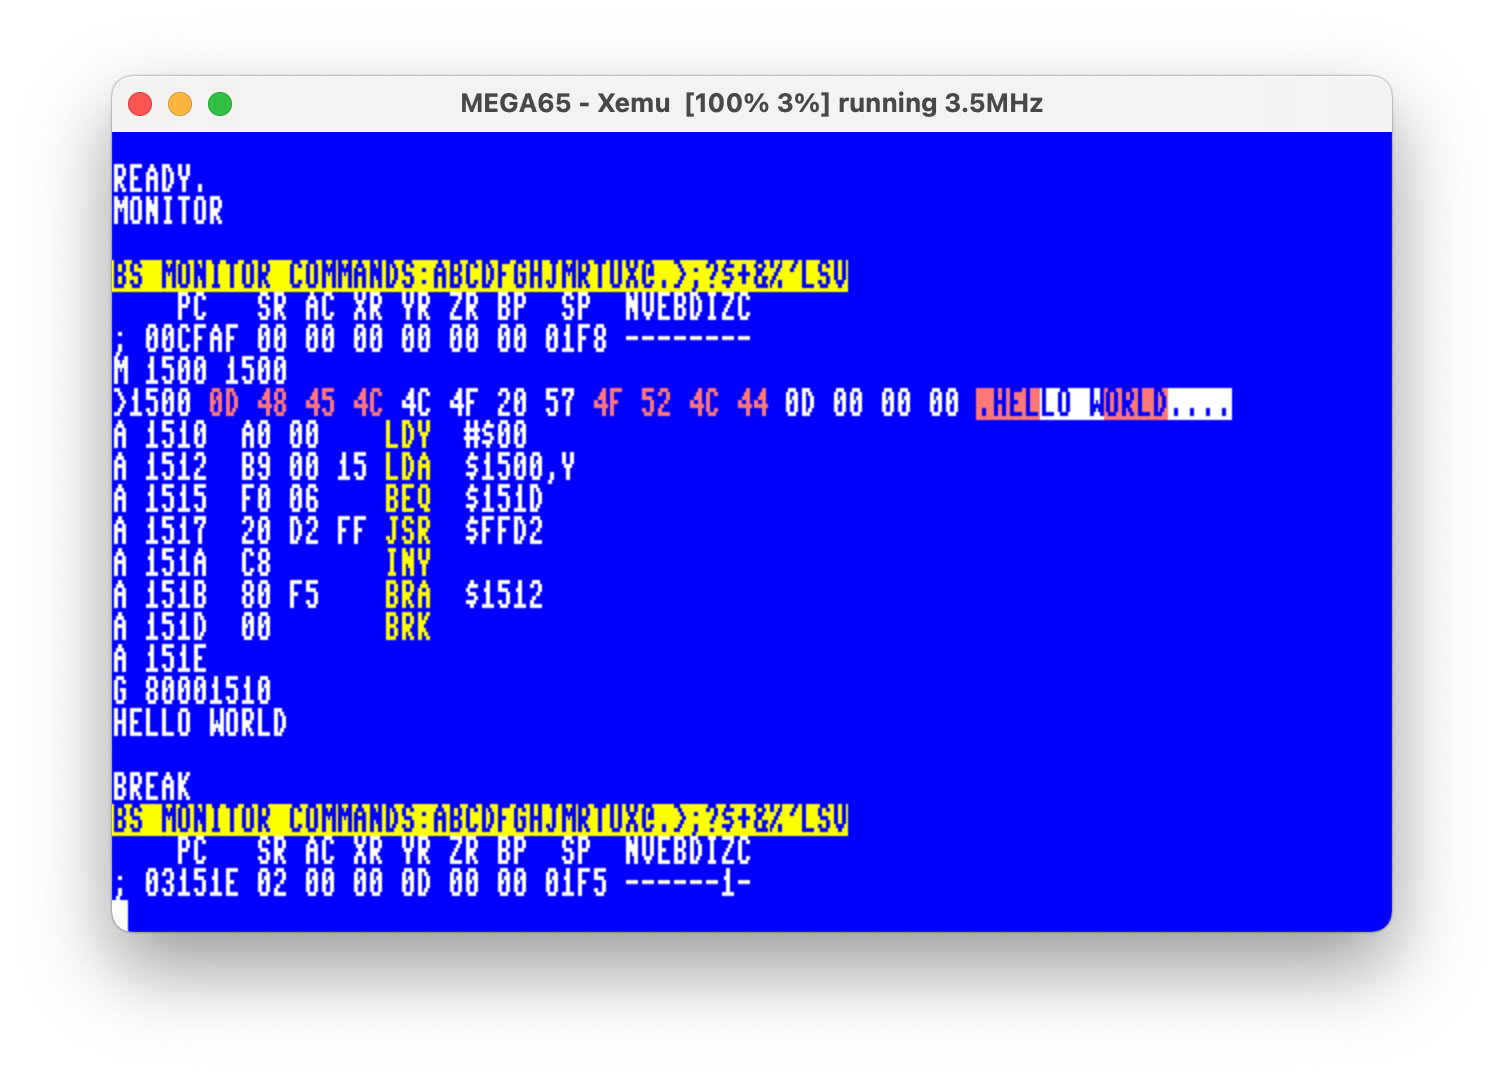
\includegraphics[width=\linewidth]{images/monitor-a}

% *******
% BITMAPS
% *******

\subsubsection{B : BITMAPS}

\index{BITMAPS}
\index{MONITOR Commands!BITMAPS}
\begin{description}[leftmargin=2cm,style=nextline]
\item [Format:] {\bf B display character bitmaps}
\item [Usage:] B address

\item [Remarks:] The B command displays the contents of memory cells bitwise
                 by printing an asterisk for 1 and a dot for 0.
                 The special arrangement of character data with 8 bytes
                 forming one character cell, is considered.
                 8 characters are displayed for each call.

                 There are three ROM character sets builtin
                 in the {\tt 92XXXX} ROMs:

\begin{tcolorbox}[colback=blue,coltext=white]
\verbatimfont{\codefont}
\begin{verbatim}
FONT A : REM $029000 : ASCII [\]^_ {|}~ included
FONT B : REM $03D000 : serif version of A
FONT C : REM $02D000 : original C64 font
\end{verbatim}
\end{tcolorbox}
\end{description}
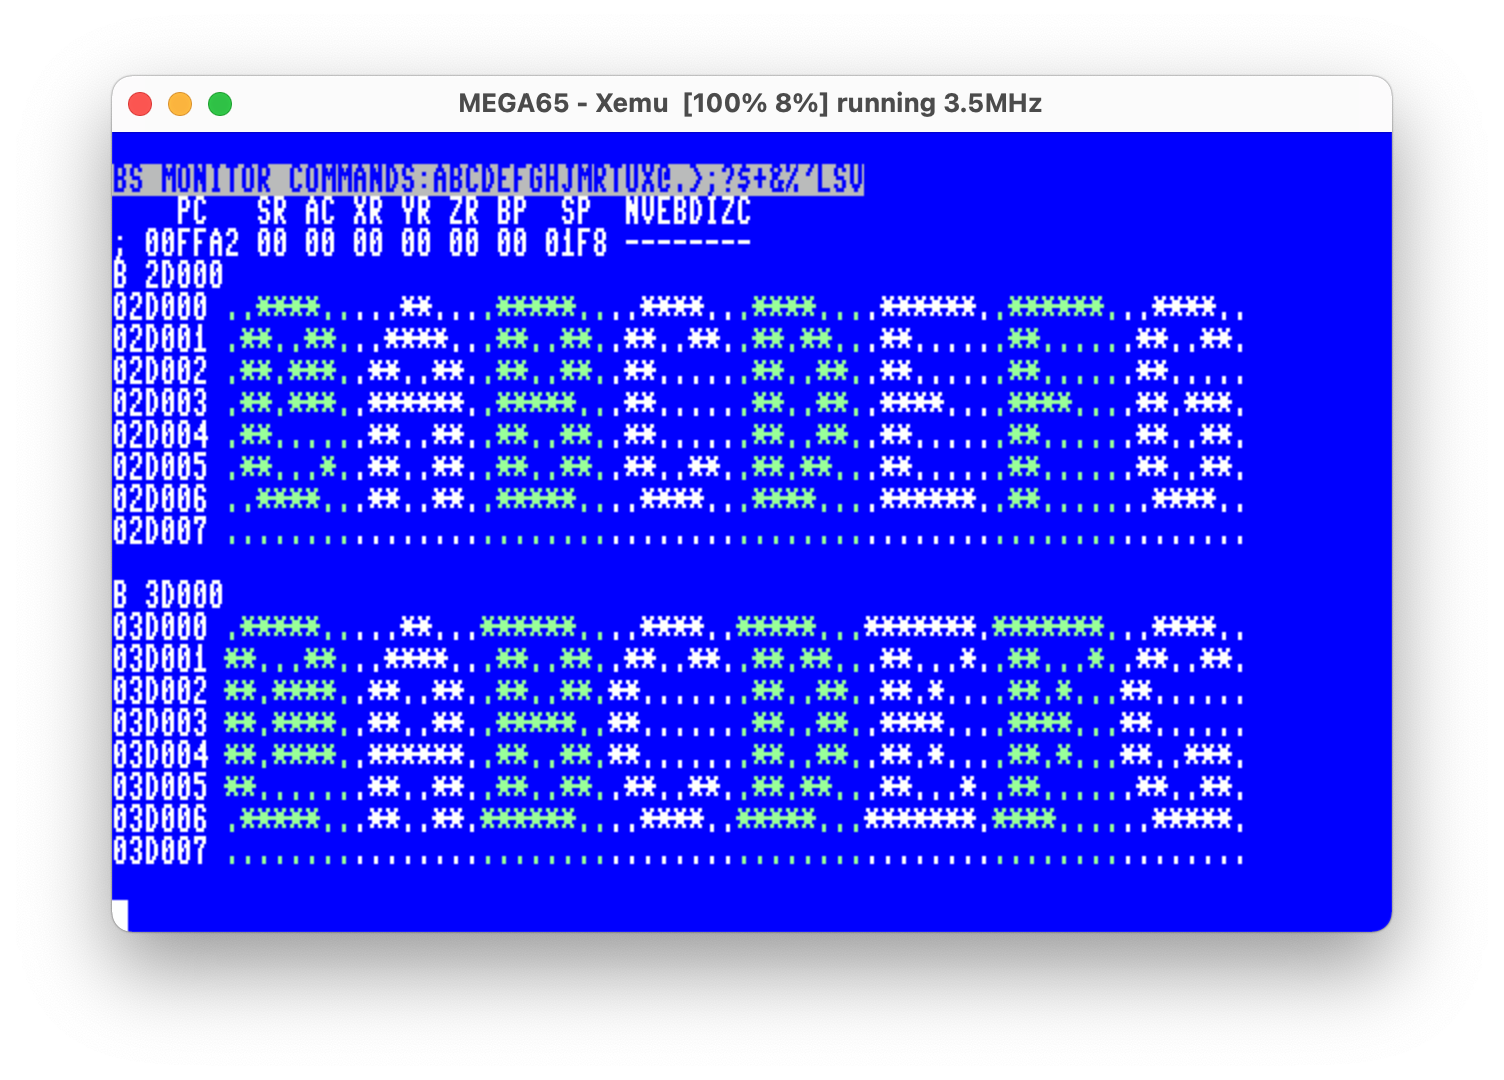
\includegraphics[width=\linewidth]{images/monitor-b}





\section{MEGA65 Matrix Mode Monitor Interface}
\index{MONITOR!Matrix Mode/Serial Monitor Interface}

This monitor is different to the other two: It is part of the MEGA65
system itself, and runs concurrently with MEGA65's processor. That is,
you can view and modify the memory the MEGA65, {\em while a program is running}.

This works using dedicated hardware in the MEGA65 design, that implements a little
helper processor that runs this monitor interface, and has a special access mechanism
to the memory and processor of the MEGA65.

In comparison with the ROM-based monitors that execute on the MEGA65's primary processor,
the Matrix Mode monitor has several advantages and disadvantages:
\begin{itemize}
\item It can be used while a program is running.
\item It can be used, even if the ROM area is being used for program code or data,
  instead of containing a standard C65 or MEGA65 ROM.
\item It can be accessed via the serial debug interface, via the JB1 connector.
\item It can be instructed to stop the processor as soon as the program counter (PC)
  register of the main processor reaches a user specified address. That is, it supports
  a (single) hardware breakpoint.
\item It can be instructed to stop the processor whenever a specified memory address
  is written to. That is, it suppors a ``write watch'' on a single memory address.
  The memory address is specified as a full 28-bit address, allowing it to detect memory
  writes via any means. Note that DMA operations will complete, before the watch point
  takes effect.
\item It can be instructed to stop the processor whenever specific CPU flags are set
  or cleared, which can also be used to support debugging of programs.
\item On some models of the MEGA65, the integrated ROM of the monitor processor is
  very small, which means that functionality may be limited. This is why, for example,
  there is no ``assemble'' command for this monitor.  This may be corrected in future
  core updates for MEGA65 models that have capacity for a larger monitor processor ROM.
\end{itemize}

\subsection{Table of Matrix Mode Monitor Commands}

{
\ttfamily
\setlength{\tabcolsep}{1mm}
\begin{center}
\begin{tabular}{|l|l|l|}
\hline
C & mnemonic & description \\
\hline
\# & HYPERTRAP & Enable/disable CPU hypervisor traps \\
+ & UARTDIVISOR & Set UART bitrate divisor \\
? & HELP & help \\
@ & CPUMEM & (show memory from CPU context) \\
\hline
B & BREAKPOINT & Set/clear CPU execution break point \\
D & DISASSEMBLE & Disassemble memory \\
E & FLAGWATCH & Set/clear CPU flags watch point \\
F & FILL & Fill memory with a value \\
G & SETPC & Set CPU program counter \\
H & HELP & help \\
I & INTERRUPTS & Enable/disable CPU interrupts \\
J & DEBUGMON & Various debug functions for the monitor itself \\
L & LOADMEMORY & Load data into memory \\
M & MEMORY & Show memory contents \\
R & REGISTERS & show registers \\
S & SETMEMORY & Set memory contents \\
T & TRACE & set CPU trace/run mode \\
W & MEMORYWATCH & Set/clear memory write watch point \\
Z & CPUHISTORY & CPU history \\
\hline
\end{tabular}
\end{center}
}

\subsection {Calling the Monitor}

To enter or exit the monitor hold down \megasymbolkey and press \specialkey{TAB}.
You will see an animation of green characters raining down from the top of the screen, and
then be presented with a simple text terminal interface which is transparent, so that you can
see the screen output of your running program at the same time.

\subsubsection{\# : Hypervisor trap enable/disable}

\index{HYPERTRAP}
\index{MONITOR Commands!HYPERTRAP}
\begin{description}[leftmargin=2cm,style=nextline]
\item [Format:] {\bf \# Enable or disable Hypervisor Traps}
\item [Usage:] \#[0|1]

\item [Remarks:] If the argument is 1, then Hypervisor traps are enabled,
  otherwise they are disabled.

  {\em It is not confirmed if this command is currently functional.}
\end{description}


\subsubsection{+ : Set Serial Interface UART Divisor}

\index{UARTDIVISOR}
\index{MONITOR Commands!UARTDIVISOR}
\begin{description}[leftmargin=2cm,style=nextline]
\item [Format:] {\bf + Set Serial Interface UART Divisor}
\item [Usage:] + divisor

\item [Remarks:] Sets the divisor for the serial monitor interface.
  This allows changing the baud rate of the serial monitor interface
  from the default 2,000,000 bits per second.  The baud rate will be
  equal to $40,500,000 \div (divisor-1)$. This affects only the
  serial UART interface, and does not affect accessing this monitor
  via the Matrix Mode composited display.

  For example, to slow the
  serial monitor interface down to 19,200 bits per second, the divisor
  would need to be $40,500,000 \div (19,200 - 1) = 2108$.
  The + command then requires that you convert this value to hexadecimal,
  thus the command would be {\tt +83c}.

  Note that this command does {\em no} sanity checking of the provided value.
  If you accidentally provide an incorrect value for your needs, you can
  recover from this situation by activating the Matrix Mode interface by holding
  down \megasymbolkey and tapping \specialkey{TAB}, and entering
  the appropriate command to correct the divisor, e.g., {\tt +14} to return
  to the default of 2,000,000 bits per second.

  You must then exit the Matrix
  Mode again by repeating the \megasymbolkey + \specialkey{TAB} key combination,
  before the serial UART interface will become active again. This is because
  the Matrix Mode disables the serial UART interface when active.
\end{description}

\subsubsection{@ : CPUMEMORY}
\index{CPUMEMORY}
\index{MONITOR Commands!CPUMEMORY}
\begin{description}[leftmargin=2cm,style=nextline]
\item [Format:] {\bf @ [address]}
\item [Usage:] Prints a memory dump for the given 16-bit address,
  {\em as interpretted by the current CPU memory mapping}.
  If you wish to inspect the contents of memory anywhere in the 28-bit
  address space, use the M command instead.

  The dump displays memory contents, organised in rows
  of 16 consecutive addresses starting with the
  address. The dump displays
  a full page of 256 bytes in 16 rows.
  The contents are printed as 16 byte values in hex,
  followed by the character representation.

\item [Remarks:] If not address is provided, it will show the next 256 bytes.

\end{description}

\subsubsection{? or H : HELP}
\index{HELP}
\index{MONITOR Commands!HELP}
\begin{description}[leftmargin=2cm,style=nextline]
\item [Format:] {\bf ?} {\em or} {\bf h}
\item [Usage:] Displays a (very) brief message identifying the monitor.
  On some models of the MEGA65 that have more memory available to the
  monitor processor, this command may display information about each
  of the available commands.

\end{description}


\subsubsection{B : BREAKPOINT}
\index{BREAKPOINT}
\index{MONITOR Commands!BREAKPOINT}
\begin{description}[leftmargin=2cm,style=nextline]
\item [Format:] {\bf b [address]}
\item [Usage:] Sets or clears the hardware breakpoint. If no address is provided,
  then the breakpoint will be disabled. Otherwise the breakpoint is set to the
  provided 16-bit address.

  Whenever the program counter (PC) register of the MEGA65's processor equals the value
  provided to this command, the processor will halt, and the Matrix Mode monitor interface
  will display the last instruction executed and current register values to alert the user
  to this event. It does not activate the Matrix Mode display when this occurs. It is
  normally expected that Matrix Mode will either already be active, or that the user is
  interacting via the serial interface.

\end{description}


\subsubsection{D : DISASSEMBLE}
\index{DISASSEMBLE}
\index{MONITOR Commands!DISASSEMBLE}
\begin{description}[leftmargin=2cm,style=nextline]
\item [Format:] {\bf <d|D> [address]}
\item [Usage:] Disassembles and displays the instruction stored at the
  indicated 28-bit address.

  To disassemble instructions from the CPU's
  current memory context, taking into account current memory banking,
  prefix the address with 777, e.g., {\tt d777080D} would disassemble
  the instruction at \$080D, as currently visible to the MEGA65's
  processor.

  Use {\tt D} instead of {\tt d} to disassemble 16 instructions at a time, instead of just one.

\end{description}

\subsubsection{E : FLAGWATCH}
\index{FLAGWATCH}
\index{MONITOR Commands!FLAGWATCH}
\begin{description}[leftmargin=2cm,style=nextline]
\item [Format:] {\bf e [value]}
\item [Usage:]
  Sets or clears the CPU flag watch point: If no argument is provided, the
  flag watch point is disabled. If a value is provided, it is assumed to be
  a 16-bit value, where the first two hexadecimal digits indicate the processor
  flags that will trigger the watch point if they are set. The second two
  hexadecimal digits indicate which processor flags will trigger the watch point
  if they are clear.  In this way any combination of processor flag values can
  be monitored.

  {\em This command does not function correctly at the time of writing.}

\item [Example:]

  To cause the watch point to trigger when the Negative Flag is asserted, the
  command {\tt e8000} would be used.

\end{description}

\subsubsection{F : FILL}
\index{FILL}
\index{MONITOR Commands!FILL}
\begin{description}[leftmargin=2cm,style=nextline]
\item [Format:] {\bf f [start] [end+1] [value] }
\item [Usage:] Fills the indicated 28-bit address range with
  the indicated value.
\item [Remarks:]
  The end address should be one more than the last address
  that is desired to be filled.

\end{description}

\subsubsection{G : SETPC}
\index{SETPC}
\index{MONITOR Commands!SETPC}
\begin{description}[leftmargin=2cm,style=nextline]
\item [Format:] {\bf g address}
\item [Usage:] Sets the Program Counter (PC) register of the MEGA65's processor
  to the supplied 16-bit address.  If the processor is running at the time, execution
  will immediately proceed from that address. If the processor is halted at the time,
  e.g., due to the use of the {\tt t1} command, the processor remains halted, but with
  the Program Counter set to the indicated address, ready for when the processor is
  again allowed to run.

\end{description}


\subsubsection{I : INTERRUPTS}
\index{INTERRUPTS}
\index{MONITOR Commands!INTERRUPTS}
\begin{description}[leftmargin=2cm,style=nextline]
\item [Format:] {\bf i[0|1]}
\item [Usage:] Enables or disables interrupts on the MEGA65's
  processor. Disabling interrupts can be helpful when single-stepping
  through a program, as otherwise you will tend to end up only
  stepping through the interrupt handler code, because the interrupts
  will happen more frequently than the steps through the code.

\item [Remarks:] {\em This command is known to have problems, and may
  not currently function.}

\end{description}

\subsubsection{J : DEBUGMON}
\index{DEBUGMON}
\index{MONITOR Commands!DEBUGMON}
\begin{description}[leftmargin=2cm,style=nextline]
\item [Format:] {\bf j [value]}
\item [Usage:] Display, and optionally set, internal signals of the matrix
  mode monitor interface.

\end{description}


\subsubsection{L : LOADMEMORY}
\index{LOADMEMORY}
\index{MONITOR Commands!LOADMEMORY}
\begin{description}[leftmargin=2cm,style=nextline]
\item [Format:] {\bf l <start addr> <end addr + 1>}
\item [Usage:] Fast-load a block of memory via the serial monitor
  interface.  Immediately after sending this command, the bytes of
  memory to be loaded should be sent to the serial monitor interface.
  The bytes are read as-is, and thus should be provided as natural
  bytes, not encoded in hexadecimal.  This allows loading data at
  approximately 200KB per second at the default serial baud rate
  of 2,000,000 bits per second.

\end{description}

\subsubsection{M : MEMORY}
\index{MEMORY}
\index{MONITOR Commands!MEMORY}
\begin{description}[leftmargin=2cm,style=nextline]
\item [Format:] {\bf <m|M> [address]}
\item [Usage:] Prints a memory dump for the given 28-bit address.
  If you wish to inspect the contents of memory as currently seen
  by the processor's current banking configuration, use the \@
  command instead.

  The dump displays memory contents, organised in rows
  of 16 consecutive addresses starting with the
  address. The dump displays
  a full page of 256 bytes in 16 rows.
  The contents are printed as 16 byte values in hex,
  followed by the character representation.

\item [Remarks:] If not address is provided, it will show the next 256 bytes.

\end{description}

\subsubsection{R : REGISTERS}
\index{REGISTERS}
\index{MONITOR Commands!REGISTERS}
\begin{description}[leftmargin=2cm,style=nextline]
\item [Format:] {\bf r}
\item [Usage:] Displays the current value of various processor registers
  and flags, as well as a disassembly of the most recently executed
  instruction.

\end{description}

\subsubsection{S : SETMEMORY}
\index{SETMEMORY}
\index{MONITOR Commands!SETMEMORY}
\begin{description}[leftmargin=2cm,style=nextline]
\item [Format:] {\bf s addr <value ...>}
\item [Usage:] Sets the contents of the indicated memory location to the supplied value.
  If more than one space-separated value is provided, then multiple consecutive memory
  locations will be set.

  This command uses 28-bit addresses, and therefore ignores the current selected memory banking
  configuration.

\end{description}


\subsubsection{T : TRACE}
\index{TRACE}
\index{MONITOR Commands!TRACE}
\begin{description}[leftmargin=2cm,style=nextline]
\item [Format:] {\bf t<0|1|c>}
\item [Usage:] Selects the trace or run mode of the processor: {\tt t0} means that the
  processor runs freely, {\tt t1} halts the processor, and {\tt tc} runs the processor
  in continuous-trace mode, where it displays each instruction and the register values
  immediately following its execution, as though {\tt t1} had been selected, and the user
  were to then immediately press return or enter to request the next instruction to be
  executed.

  If {\tt t1} is selected, pressing enter or return in the Matrix Mode monitor will cause
  the next instruction to be executed.

  The {\tt t0} command is also used following the triggering of a break-point or watch-point,
  to allow the processor to resume.

\end{description}

\subsubsection{W : WATCHPOINT}
\index{WATCHPOINT}
\index{MONITOR Commands!WATCHPOINT}
\begin{description}[leftmargin=2cm,style=nextline]
\item [Format:] {\bf w [address]}
\item [Usage:] Sets or clears the hardware watch-point. If no address is provided,
  then the watch-point will be disabled. Otherwise the watch-point is set to the
  provided 28-bit address.

  Whenever the MEGA65's processor writes to the address
  provided to this command, the processor will halt, and the Matrix Mode monitor interface
  will display the last instruction executed and current register values to alert the user
  to this event.  It does not activate the Matrix Mode display when this occurs.
  It is
  normally expected that Matrix Mode will either already be active, or that the user is
  interacting via the serial interface.

\end{description}

\subsubsection{Z : CPUHISTORY}
\index{CPUHISTORY}
\index{MONITOR Commands!CPUHISTORY}
\begin{description}[leftmargin=2cm,style=nextline]
\item [Format:] {\bf z [address]}
\item [Usage:] Displays information about the instructions recently executed by
  the MEGA65's processor.

\item [Remarks:] {\em This command is suspected to not be correctly operational at
  the time of writing.}

\end{description}




